\chapter{One Layer}
\label{chap:singleLayer}

{\em *** Version: \today~ ***}

%reorganizing Chapter 5

Introduction

Proxima is levels with layers in between.
Here we specify the types of the levels, and what functions between them.

The defs hold for all layers and levels, although some special cases.

Renderer is implemented as tree, but

\section{5.1 Defs?}
Level, Layer

\section{5.2 The Presentation and Interpretation invariants}

\section{5.3 Upward and downward mappings at one layer}
 Info on nature of the mappings between two levels
   \subsection{3.1 The presentation mapping}
   \subsection{3.2 The interpretation mapping}
   \subsection{3.3 Duplicates in presentation}
    does this belong here?
    
\section{5.4 Extra state}
 say some things about level. It consists of several parts. 
 
   \subsection{4.1 Extra state in presentation and interpretation direction}
      
   \subsection{4.2 One level has two kinds of extra state}
      SPEC 1: LEVELs
   \subsection{4.3 Mapping information}
      SPEC Final: LEVELs

\section{5.5 Maintaining the presentation invariant during editing}
                   Specification of a single layer
   \subsection{5.1 Presentation and interpretation sheets}
      SPEC 1: Layer
   \subsection{5.2 Maintaining extra state}
                           Specification with extra state?
      SPEC 2: Layer
   \subsection{5.3 Safety of extra state}
   \subsection{5.4 Conclusions}

\section{5.6 Incrementality}
   \subsection{6.1 From a mapping between levels to a mapping between edit
operations}
   \subsection{6.2 Shorthand notation for level updates}
   \subsection{6.3 Maintaining the presentation invariant}
                  Final specification
        SPEC Final: Layer
\section{5.7 Conclusions}










\bc
Edit is overloaded, is this okay?


?? mention that in the process of refinement, only the last step makes sense? Direct/indirect edit ops etc. from previous chapters is not made here, and breaks invariants. Will (hopefully) be fixed in next chapter.


Duplications somewhere else? Only in evaluator.
mapping toc, two arrows, one to each group
be clear on when mapping is required. Only if lower has ls. back only if partial pres?



TODO
check super & subscripts in figures and text: h/high h,intr or h_intr, etc.

SOMEWHERE: mappings important for extra state, but also for editing on several levels. (is this really true?)

MAPPING INFO INCONSISTENCY: figure out how to express that two cycles are needed to restore it.
                                                  %is probably related to edit ops starting at higher level
ALSO ALL IS ON TREES, for other things, eg, sum of leafs, it does not work, do it yourself
EXTRA STATE, also tree ordering? precedence op tree -> non ordered op tree?
SOMEWHERE, explain why this is all necessary, refer to Editing Chapter


***EXTRA STATE is based on invariant mapping, however, implemented mapping is from level to level
***EXTRA STATE is only possible when inc. because lev, cannot be derived, or maybe only store extra?

** SOMEWHERE. pres is typically just for viewing: no big problem when destroyed
** intr is more essential. bigger problem when destroyed.
** guarantee no loss, so only limited edit func. on toc.

interpretation is bit strange as edit ops can be on higher level
* could this also be the case with presentation?


!!!!!!!!!
MAYBE we want to make Present and Interpret the intended and specified mappings, 
without extra stuff and mappings, then the editor has to implement the incremental ones
 and mapping preserving things, so the result is that Present and Interpret hold.
- this is what we do now

!however, in that case Present.Interpret will not be id if Present is ambiguous, or 
has extra state. But maybe we don't care and only require the implementation to be id.

!what about sheets? 

SOMEWHERE: FOCUS more formally (if included then add forward refs to edit model chapter)


IMPL: mapping downward, how to store in doc? Now datatype changes when pres is modified

\ec


%* explain edit steps? Before fitting it all together, we first build one layer

In the layered architecture of Proxima (see Chapter~\ref{chap:proxArch}), each layer maintains invariants between two adjacent levels. When either the higher or the lower level is changed, the other adjacent level is updated apropriately. The process of updating the levels is largely symmetrical for both directions.

This chapter discusses the invariants that are maintained between two adjacent levels from the perspective of a single layer. Furthermore, it specifies the additional information necessary for computing the updates that restore the invariants. The invariants given in this chapter hold for any layer in the Proxima system, although several layers will be simpler than the generic layer presented here.

Besides the abstract invariants, we also present a specification of the concrete functions that need to implemented in order to maintain the layer invariants. The single layer specification serves as a basis for the specification of an entire editor in the next chapter, when the layers are connected.


% based on a mapping between levels
% add sheets, add extra and add incrementality

\note{somewhere: Stress that mappings are not needed when for subtrees for which the lower level is not editable}
\note{somewhere: Stress that it's only an architecture. Safety, impl. etc is left to layer. Future research (Pierce?)}
%rather than safe toy, complete arch for many ed's Safety and patterns need to be researched

\bc
Where say that mapping back is only when we need automatic editing: is it only important for duplicates? It seems to be important for 2:1 presentations as well.  In some complicated cases, the mapping back cannot be spec'd if mapping back is does not work, it means that lower edit cannot be handled, and is forbidden. However, we always have the higher level edit left.
\ec


%																
%																
%																
\section{Defs?}

some defs + what we are going to do.

Relation to rest of proxima

Level

Layer


%																
%																
%																
\section{The Presentation and Interpretation invariants}

% will become more a computation order

Because in this chapter we only look at a single layer, there are only two data levels to take into account: a higher level ($\level_{H} :: \Level_{H}$) and a lower level ($\level_{L} :: \Level_{L}$). The two levels are related by two invariants: the {\em presentation invariant} and the {\em interpretation invariant}. 

The presentation invariant is satisfied if and only if the lower level is a correct presentation of the higher level. The invariant is expressed using an abstract function 
$\Present ::  \Level_{H} \rightarrow \Level_{L}$.

\begin{small}\begin{math}
\text{\bf Presentation invariant:~~~} \level_{L} = \Present~\level_{H}\\
\end{math}\end{small}

Similarly, the interpretation invariant is satisfied if and only if the higher level is a correct interpretation of the lower level. The interpretation invariant is expressed with a function 
$\Interpret ::  \Level_{L} \rightarrow \Level_{H}$.

\begin{small}\begin{math}
\text{\bf Interpretation invariant:~~~} \level_{H} = \Interpret~\level_{L}\\
\end{math}\end{small}

$\Present$ and $\Interpret$ are not actual functions that can be evaluated, but abstract concepts used to express a property of two levels. The functions are used to specify the behavior of a layer.
Strictly speaking, $\Present$ and $\Interpret$ are not even functions but relations, since a higher level may have several correct presentations, and a lower level may have several correct interpretations. However, this occurs only if a level has extra state, as will be explained in Section~\ref{sect:extraState}.

Because we only look at one layer in this chapter (ie. the layer between $\Level_{H}$ and $\Level_{L}$), we need two more functions to refer to the behavior of the layers below this layer, as well as the layers above. For lower layers, the function $\Edit :: \Level_{L} \rightarrow \Level_{L}$ denotes an update on $\Level_{L}$ by the lower layers. For representing updates on the higher level, we use 
$\Transform :: \Level_{H} \rightarrow \Level_{H}$. In the next chapter, when layers are connected, $\Edit$ and $\Transform$ become superfluous.

Figure~\ref{layerEditProcess} shows how the invariants are used to specify the data level updates that occur in a single edit step. On the left-hand side are the levels and layers of Proxima, during one edit step. One of the layers is shown separately on the right. 

The precondition before the edit operation takes place is that the lower level is a correct presentation of the higher level, that is $\level_{L} = \Present~\level_{H}$. In the levels below, an edit operation takes place, which results in an updated lower level: $\level'_{L}$. Because the presentation invariant will not necessarily hold anymore, an appropriate higher level is specified by the interpretation invariant:
$\level'_{H} = \Interpret~\level'_{L}$. The new higher level is then processed by higher layers, resulting in the final higher level value for this edit step: $\level''_{H}$. Finally, the postcondition is established by updating the lower level to $\level''_{L}$ for which 
$\level''_{L} = \Present~\level''_{H}$ holds. 

The successive updates on the levels can be expressed with equations:

\begin{small}\begin{math}
\level_{L} = \Present~\level_{H}	\hfill \text{\{Precondition\}}\\
\level'_{L} = \Edit~\level_{L}		\hfill \text{\{User edit\}}\\
\level'_{H} = \Interpret~\level'_{L}	\hfill \text{\{Intermediate condition\}}\\
\level''_{H} = \Transform~\level'_{H}\hfill \text{\{Higher layer update\}}\\
\level''_{L} = \Present~\level''_{H}	\hfill \text{\{Postcondition\}}\\
\end{math}\end{small}

% can we express when this happens with a condition? pres .. /= pres .. oid?
The reason why $\level'_{H}$ is not immediately presented, is that it first has to be processed by the higher layers, just as $\level'_{L}$ is processed by this layer. The final value $\level''_{H}$ may be equal to $\level'_{H}$, but certainly does not have to be. Take an enriched document that contains a list of numbers together with the sum of the numbers. When one of the numbers is edited at the presentation level, the new enriched document that results from parsing ($\level'_{H}$) is a list of numbers together with a sum value that is most likely to be incorrect. In order to compute the a sum value, the enriched document needs to be passed on to the reducer and evaluator, resulting in a final enriched document ($\level''_{H}$) that reflects a correct sum.

\begin{figure}
\begin{small}
\begin{center}
\begin{center}
\epsfig{file=pics/eps/layer.eps, height=1.7in}
\end{center}\caption{An edit step on one level.}\label{layerEditProcess} 
\end{center}
\end{small}
\end{figure}

% why two:
We use two invariants instead of one, to make it possible to describe the intermediate state in which changes have not been fully propagated upwards and been taken into full account. Consider an editor in which an enriched document node for a product expression (\verb|Product (Int 1) (Int 2)|) is presented as a list of presentation level tokens, colored according to the syntax. The integer values are presented in black, and the operator in green. If we denote the colors between braces, the presentation is \verb|["1" {black}, "*" {green}, "2" {black}]|. Because the presentation level is a correct presentation of the document level, the presentation invariant is satisfied. But now consider a list of tokens typed by the user, which do not have the correct coloring: \verb|["1" {black}, "*" {black}, "2" {black}]|. If we use a single invariant, then expressing that \verb|Product (Int 1) (Int 2)| is an appropriate interpretation of the uncolored tokens list, also implies that the uncolored tokens are a correct presentation of the product expression. It is no longer possible to express that the colored presentation is a correct presentation of the product, whereas the uncolored presentation is not. \note{are we saying that with one invariant, pres is inverse of intr?}

\bc
\note{mention that these things need to be each other's inverse}
******** NOT TRUE, this will appear somewhere more downward, probably in ES section
The functions $\Present$ and $\Interpret$ are closely related, but in contrast to what the types might suggest, the functions are in general not each others inverse. Because interpreting a presented document should not change the document, we do have: 

\begin{small}\begin{math}
\Interpret \oo \Present = id_{H}
\end{math}\end{small}

\note{what about ambiguity?}

However, the reverse ($\Present \oo \Interpret = id_{L}$) does not necessarily hold. The condition implies that an edited lower level does not change when it is interpreted and presented \note{also say that higher layers should not change it?}, which is not always true. The syntax coloring example provides a case in which it does not hold; if an uncolored presentation is interpreted and then presented, the result is a colored presentation. 
\note{pres is injective, and intr isn't?}
\ec

%summary
Summarizing, the {\em Presentation} invariant specifies that two levels are in a final state, in which the lower level is a correct presentation of the higher. When the lower level is updated, the {\em Interpretation} invariant specifies a correct new higher level, which is passed on to the higher layers. From the higher layers, we get a final value for the higher level (for this edit step), for which a correct final lower level is specified by the {\em Presentation} invariant. The layer in between each pair of levels takes care of maintaining the invariants by invoking functions that compute level updates that reestablish the presentation and interpretation invariants.

\note{say something about Interpret.Present here as well?}

\bc
?present~sheet~.~interpret~sheet = id_{H}\\

OTHER EXAMPLE?: Apart from the syntax coloring example, the problem also arises when for example a textual arrow 
\verb|"->"| is presented as a $\rightarrow$. 

Vice versa? Fix by remembering extra?
 layer shortcutting can now be expressed by only letting the lower pres invariants hold

 -explain that in incremental, present and interpret cannot be used instead of Present and Interpret
 -how does this relate to inc with diff etc. maybe that can be expressed nicely with Present
 (or even present, then Present will be superfluous.)

* does   intr.pres = id hold for a layer? pres.intr never needs to hold due to syntax coloring, normalization etc., but also because Chess board is not a presentation of ChessBoard   
* intr.pres = id? then each pres has unique doc. Is this true? Can't doc variants be presented as same thing?
   present( interpret uncolored ) = colored, so present.interpret /= id
   interpret ( present ) = id? if so, what if two docs are presented on the same pres?
 it seems true, interpret.present cycles should not alter the doc. In case of ambiguity, the system should
 take care of conservative behavior. On an edit, the doc may change, but that's not a (interpret.present) cycle

****** When this is figured out, update sheet paragraph
\ec


%																
\section{Upward and downward mappings at one layer}\label{mappingsInLayer}

% mapping is relation levelH levelL but each two levels express a mapping between nodes.

On presentation and interpretation, elements in one data level are mapped onto elements in another level. Hence, when either the presentation or the interpretation invariant holds between two levels, we also have a mapping between the tree nodes of these levels. 

Figure~\ref{nodeMapping} shows an example of such a mapping between two levels. The dotted arrows denote on which lower level nodes a higher level node is mapped and vice versa. To reduce the number of arrows in the figure, the lower level nodes are grouped.

\bc The presentation and interpretation invariants are expressed using two functions\note{incorrect:relations}: $\Present$ and $\Interpret$. The functions are of type $\Level_i \rightarrow \Level_j$ (where $j = i+1$ or
$j = i-1$), which means that both functions map a tree onto another tree. However, since a tree structure consist of nodes, we can also view each mapping as a mapping between the nodes of one tree and the nodes of another tree. \note{do we put a restriction on the possible mapping functions with this?} 
\ec

By mapping between tree nodes, we mean a mapping that relates only the nodes and not the subtrees rooted at theses nodes. We can see this in Figure~\ref{nodeMapping}, by the fact that a child of a lower level node is not necessarily inside the same dotted ellipse as its parent. \note{also say that higher level child {\em cannot} be in same ellipse?}


A difference between the presentation and interpretation mappings, is that the presentation of a higher level node may consist of several lower level nodes, whereas the interpretation of a lower level node may consist of at most one higher level node. This is why the nodes on the right side (the lower level) are grouped together with dotted ellipses, whereas the nodes on the left side are not. The reason for the distinction is that 
\toHere     % ^^^^^^^^^^^^^^^^^^^^^^^^^^^^^^^^^^^^^

DISCUSS: is this restriction necessary? Or could we have n:m mappings?
% restriction is on presentation. pres is like a fold
% iets algemener verhaaltje hier. over dat het wel kan, maar dat de
% automatische dingen (focus etc.) dan weg zijn

AG automatically does it, but do we need to enforce? What about focus, is that the reason?
Parser makes it hard to do n:m reuse. So implementation suggests the 1:n. Maybe lift when we know how. For eval layer might be possible already. Right now only one is responsible.  Only that one can be reused and therefore may have ES (color example, only string is reused). IntExp Int example, IntExp no pres elts, so no ES. (bit different again, since Int is entire presentation, unlike String Color example) 
**
\fromHere  % VVVVVVVVVVVVVVVVVVVVVVVVVVVVVVVVVVVVVVVVVVVV


\bc
Hence, when an element \verb|A| is mapped onto an element \verb|B|, this does not say anything about the children of \verb|A| and \verb|B|. If \verb|A| is mapped onto \verb|B| including its children, this is mentioned explicitly. In Figure~\ref{nodeMapping} element \verb|aH| is mapped onto the elements \verb|a1L|,\verb|a2L|, and \verb|a3L|, so in this case the children of \verb|a1L| are included in the mapping, but the children of \verb|a2L| and \verb|a3L| are not. 
\ec

\bc
When regarded as relating tree nodes, a mapping can express an $n:m$ relation between the nodes of the higher and the lower levels. However, when regarded as relating levels, a mapping is always a function (ie. an $n:1$ relation). Thus, $\Present$ and $\Interpret$ are functions rather than relations.
\note{WITH ES, they are relations!}
\ec

\begin{figure}
\begin{center}
\begin{center}
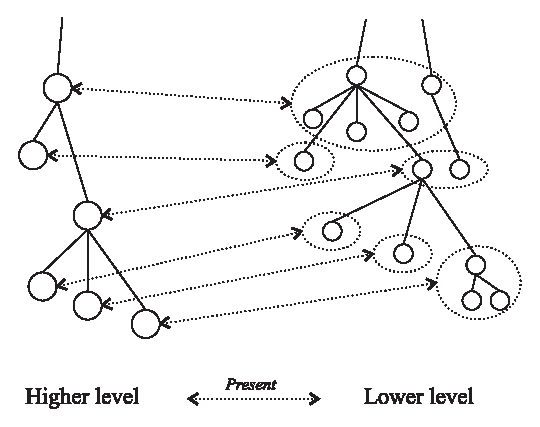
\epsfig{file=pics/eps/mapping.eps, width=2in}
\end{center}
\caption{A mapping between the nodes of two levels.}\label{nodeMapping} 
\end{center}
\end{figure}



%																
\subsection{The presentation mapping}

\begin{figure}
\begin{center}
\begin{center}
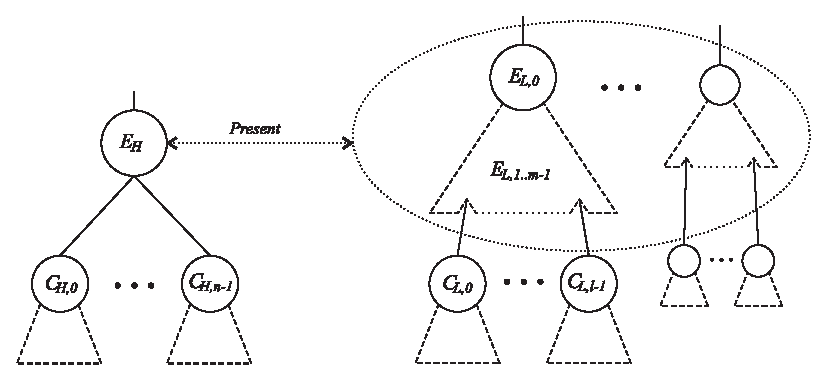
\epsfig{file=pics/eps/presentationEh.eps, width=80mm}
%\begin{verbatim}
%                  ..
%                    \
%..                   EL0
%  \                 ELEL.
%   EH       ->     EL..EL.
%  / \             EL....EL. 
% C...C           EL......EL.
%                EL/\EL.EL/\EL.
%                 /__\   /__\
%                    
%\end{verbatim}
\end{center}
\caption{The presentation of element $E_H$.}\label{elementPresentation} 
\end{center}
\end{figure}

First we take a closer look at the downward, or presentation, direction. $\Present$ relates each element of the higher level onto zero or more lower level elements, forming zero or more subtrees with holes. \note{is there a name for 'tree with holes'? eg. 'tree segment'?} Figure~\ref{elementPresentation} schematically shows the presentation of a node ($E_H$) in the higher level. $E_H$ has $n$ children ($C_{H,0\dots n-1}$). The presentation of $E_H$ is a number of trees (although usually just one) that may consist of several nodes. In the figure, the first tree is shown in more detail. It consists of $m$ nodes ($E_{L,0\dots m-1}$), is rooted at $E_{L,0}$. 

The $C_{L,0}$, \dots, $C_{L,l-1}$ subtrees in the lower level tree are not part of the presentation of $E_H$. Typically, these are the presentations of the children of $E_H$, but in general they can be (part of) the presentation of any element in the higher level. Alternatively, if a subtree is not a presentation of any higher level element, it is part of the extra state of the lower level, something that will be explained in the next section.

\begin{figure}
\begin{center}
\begin{center}
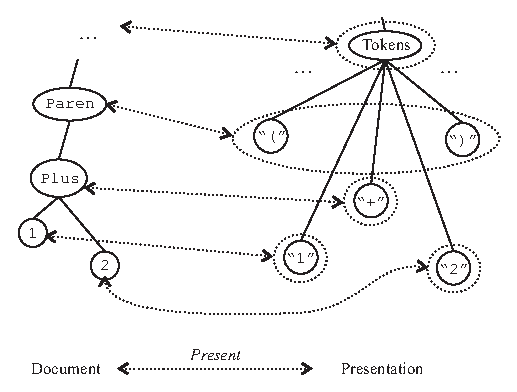
\epsfig{file=pics/eps/presentParenSum.eps}
%
%  ( )       Tk   ( 1+2 )
%   +      Tk ...
%  1 2       .....  
%
\end{center}
\caption{The presentation of a parenthesized sum.}\label{presentExample} 
\end{center}
\end{figure}

Figure~\ref{presentExample} provides a more concrete example of a presentation, taken from a source editor (see Section~\ref{sect:sourceeditor}). A parenthesized sum in the enriched document is presented as a set of tokens on the presentation level. The figure shows only a fragment of the enriched document and its presentation. \bc , leaving out the tokens to the left and the right of the expression, as well as the origin of the Tokens element. \ec The tuples in the presentation represent the whitespace of the tokens (line breaks, spaces) as defined in Section~\ref{sect:presLevel}. To the editing user, the expression will appear as "{\tt (\textvisiblespace 1+2\textvisiblespace )}". No arrows point toward the tuples, because white space is extra state of the presentation level (see Section~\ref{sect:extraState}). 

\bc
In the example, the resulting presentation is a single tree, but this is not always the case. For example, the evaluation layer in a word processor (see Section~\ref{sect:wordprocessor}), maps each chapter onto an entry in the table of contents, as well as onto the presentation of the chapter itself. Hence, the presentation (in this case the evaluation) of a chapter consists of two separate enriched document trees.
\ec



%																
\subsection{The interpretation mapping}

The upward direction, or interpretation, is slightly more restricted than the downward direction, because a lower level element is allowed to be mapped onto at most one higher level element. \note{do we want this restriction?} Figure~\ref{elementInterpretation} schematically shows an interpretation of a number of subtrees rooted at $E_L$. The children in the lower level tree are not mapped onto $E_H$. Typically, a child of $E_L$ is mapped onto a child of $E_H$, but it is also possible that it is mapped onto another higher level node, or ignored altogether in the interpretation mapping (extra state).  Again, the lower level structure is not necessarily a single subtree (with holes); it may consist of several subtrees as the next example shows.

Figure~\ref{interpretExample} contains an interpretation example. The presentation is a list of tokens of which only three tokens (\verb|"if"|, \verb|"then"| and \verb|"else"|) are shown. When parsed, the three tokens are mapped onto a single enriched document \verb|If| node. 

\begin{figure}
\begin{center}
\begin{center}
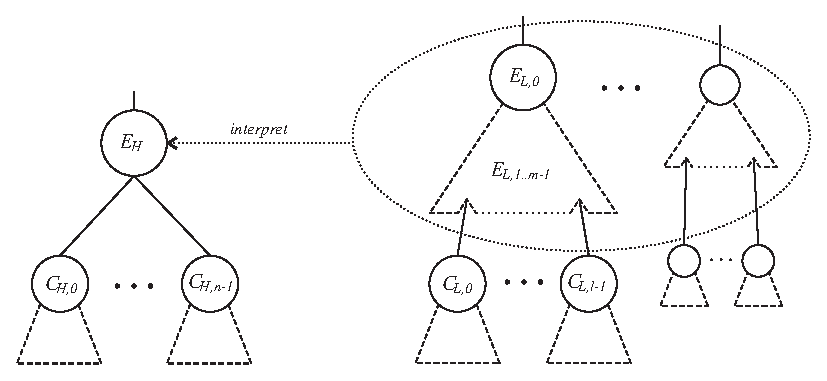
\epsfig{file=pics/eps/interpretationEl.eps, width=80mm}
%\begin{verbatim}
%
%        EL                 ->    EH
%    EL.......EL               CH ..  CH
% EL  CL  EL  CL  EL
%
%\end{verbatim}
\end{center}
\caption{The interpretation of the tree rooted at {\tt EL} (beetje dubbel?)}\label{elementInterpretation} 
\end{center}
\end{figure}


\toHere     % ^^^^^^^^^^^^^^^^^^^^^^^^^^^^^^^^^^^^^

\begin{figure}
\begin{center}
\begin{center}
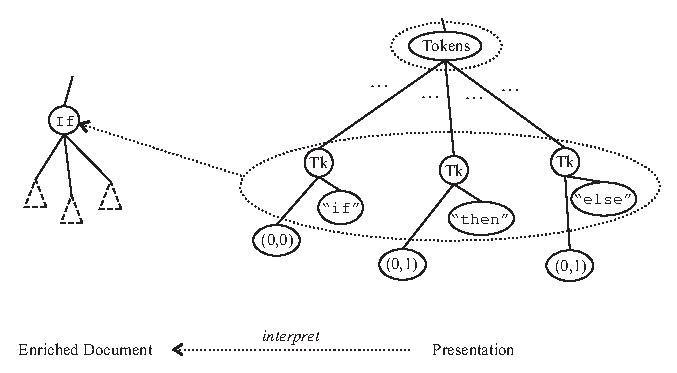
\epsfig{file=pics/eps/interpretIf.eps}
\end{center}
\caption{The interpretation of an if expression.}\label{interpretExample} 
\end{center}
\end{figure}

A consequence of the difference between the presentation and the interpretation mappings is that even when a lower level element depends on several higher level elements, only one is responsible for its presentation. For example, when an element \verb|Word Color String|, representing a colored string, is presented as a string in the specified color. Now the string in the presentation is presentation of \verb|Color| as well as of \verb|String|. However, only one of the two can be the interpretation of the . In order to edit the color


  \note{where does this become important?} \note{example: leaf Color Int $\rightarrow$ colored int. When selecting, either lead or int,  Color affects but is not responsible. can be accessed by special edit ops though.}
\note {maybe say something about 1:n presentation restriction, but also about having $>$1 doc nodes influence same pres.? Or before?}

******** PROBLEM With IntExp  Int. 
Is IntExp interpretation ES (Then ES is not always a subtree, but can be a segment as well: Paren -- IntExp(es) -- Int )? Then reusing is not as easy anymore.\\
Or can interpretation map onto 2 nodes after all?\\
Or do we just ignore elts with no pres and rebuild them when interpreting?\\
Need more experience



**** say more on Present . Interpret and Interpret . Present? Is a bit hard since they are not functions.

\fromHere  % VVVVVVVVVVVVVVVVVVVVVVVVVVVVVVVVVVVVVVVVVVVV

%\toHere     % ^^^^^^^^^^^^^^^^^^^^^^^^^^^^^^^^^^^^^
%
%
%*what about parsing to something double?
%*what about IdExp (Id "a")    ->   "a"
%*Isn't this too restrictive?
%* doesn't this make the presentation more simple? interpretation is hard because several elements need to be 
%regarded.
%if we propagate a value downward as an attribute, it already happens.
%\fromHere  % VVVVVVVVVVVVVVVVVVVVVVVVVVVVVVVVVVVVVVVVVVVV


%* if then else? tokens as list? then focus does not work (no?). tokens as tree?



%																
\subsection{Duplicates in presentation}

\note{mention duplicates in interpretation?}
\note{mention that this can also be used for multiple views?}
%* not just because multiple trees: elements may depend on several trees. without duplication.

The presentation of a higher level element may consist of several lower level elements, as shown in in Figure~\ref{interpretExample}. In this case, the \verb|If| node is the interpretation of all three tokens together. However, it is also possible that a higher level element is duplicated in the presentation, in which case interpretation of the lower level may yield conflicting values for the higher level element. An example of such a duplication is the title of a chapter that appears in the table of contents as well as in the presentation of the chapter itself. When the lower level is interpreted, several alternatives for one element may arise, and a choice has to be made.

Note that having several lower level elements does not automatically mean that an element is duplicated. Furthermore, the interpretation of duplicates only needs to be dealt with if the duplicate structure is edited on the lower level. If a duplicate only needs to support document editing and no presentation editing, no extra work needs to be done.

The only two layers suitable for specifying duplicates are the evaluation and the presentation layer. The presentation mappings for the other layers are largely predefined and do not duplicate any structures. To avoid having to deal with duplicates when parsing, duplicating is currently only allowed at the evaluation layer. This restriction may be lifted in a future version, but for now, if a presentation contains duplicates, the evaluation sheet specifies how the involved structures are duplicated, and the reduction sheet specifies how updates on duplicate structures are handled.

\begin{figure}
\begin{center}
\begin{center}
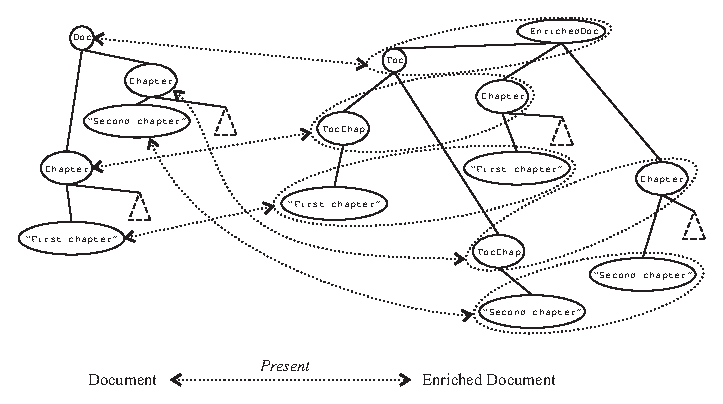
\epsfig{file=pics/eps/interpretToc.eps}
%
%  Chap              Toc
%  "first.."     TokChap      Chap
%                   "first.."     "first.." 
%
\end{center}
\caption{The interpretation of a word processor document with a table of contents.}\label{duplicatesExample} 
\end{center}
\end{figure}

Figure~\ref{duplicatesExample} shows an example of a duplicated structure in the form of a table of contents for a word processor. On the left-hand side of the figure is a document that contains two chapters, of which only the titles are shown. The enriched document contains both a table of contents subtree (\verb|Toc|), as well as a copy of the chapters. The table of contents subtree follows the structure of the original document, but only contains the title of each chapter rather than the chapter itself. To keep the figure simple, the table of contents only contains chapters and not sections and subsections, but in a real editor the table of contents may reflect the entire document structure. 

The evaluator maps a chapter in the document on a chapter in the enriched document, as well as on a chapter entry in the table of contents tree, in the latter case leaving out everything but the title. The presenter simply presents both the table of contents tree as well as the chapter tree, and does not duplicate any structures. The table of contents example is somewhat complex, because it does not only involve a duplicated presentation, but also a partial presentation (a chapter in the table of contents is shown without its content). Section~\ref{sect:extraState} discusses how partial presentations are handled.

When the enriched document is edited it is interpreted (reduced), yielding an updated document. For duplicate structures, the enriched document contains several alternatives, which may have different interpretations. In the table of contents example, the alternatives for a chapter title are the title in the table of contents and the title in the chapter. Three situations are possible. Firstly, if none of the alternatives have been edited, all interpretations are equal, and any one can be chosen. Secondly, if one alternative has been edited, the choice is in favor of the edited element. Hence, if a chapter title is edited in the table of contents, the resulting reduced document contains the updated title. Finally, if more than one value has been edited, an error is signaled to the user. In the example, this happens when the title is edited in the chapter as well as in the table of contents. In this case the edit operation may be forbidden, or either one of the values may be chosen.  \note{say that we cannot skip the evaluation layer with this scheme?}

Specifying duplications in the evaluation and reduction sheets is not ideal, since the enriched document type now depends on whether or not the presentation contains duplicates. Hence, if a presentation contains several views on a structure, the necessary duplications for these views need to be specified in the evaluation layer. A special facility in for specifying common duplicate presentations, such as tree views on a structure, in the presentation layer is desirable. A possible approach for such functionality is a special parser that can resolve conflicts duplicates during parsing. With such a parser, the entire process of handling duplicates takes place in the presentation layer, and the evaluation layer is not affected. \note{parse (dirty arrangement) $\rightarrow$ dirty presentation? May be tricky as well}

%																
%																
%																
\section{Extra state} \label{sect:extraState}

%SOMEWHERE: when es is hard. If no parent with a presentation is parent then 
% tricky. Hence invisible elements with extra state may lose it during editing.

\note{specify conditions for safety? like in Pierce's lenses stuff?}
\note{mention Pierce paper?}

In some cases, a lower level contains information that cannot be computed by presenting its adjacent higher level. Similarly, a higher level may contain information that cannot be computed by interpreting the lower level. The information in a level that cannot be computed by presenting, or interpreting an adjacent level, is referred to as {\em extra state} (also see sections~\ref{sect:editingExtraState}~and~\ref{sect:archExtraState}). Because extra state cannot be computed by the mapping function, its previous value is reused, if possible. In this section, we refine the definitions of the data levels in order to give a more precise definition of this extra state. Furthermore, we specify what information needs to be kept track of in order to handle extra state.


%This section gives a more precise definition of extra state and specifies how  Furthermore, 
%This section explains : welke info. wanneer gaat het mis. 


%																
\subsection{Extra state in presentation and interpretation direction}

\bc
during is not okay+ levels benoemen, want er wordt vaak heen en weer gesprongen.

% One layer: two kinds of extra
Since a presentation of an element may consist of zero or more elements, and an interpretation consists of at most one, it is possible that an element is not mapped onto any elements in the target level. In that case, the target level simply does not contain the information needed to compute the element**iets specifieker**, and hence it ** what ** is part of the former level's extra state. Because whether or not a node is extra state depends on which mapping we consider, we distinguish two kinds of extra state: presentation extra state and interpretation extra state. The {\em presentation extra state} consists of elements that during presentation cannot be computed from the higher level (the shaded elements at the top level of Figure~\ref{layerExtraState}), and the {\em interpretation extra state} consists of elements that during interpretation cannot be computed from the lower level (the shaded elements at the bottom layer of the figure).
\ec


% example pres extra
Figure~\ref{layerExtraState} shows two examples of extra state, one occurring on presentation, and the other on interpretation. On the left-hand side, an enriched document node is presented as a token. The shaded whitespace node (0,1) is not specified by the presentation mapping, and hence is part of the lower level {\em presentation extra state}. On presentation, tokens are reused, causing the whitespace information to stay the same. In order to do this, we need to know exactly on which presentation elements an enriched document node was mapped when it was previously presented. In case a token has no previous whitespace, for example because it is the presentation of an enriched document part that has not been presented before, a default value is used.

\begin{figure}
\begin{center}
\begin{center}
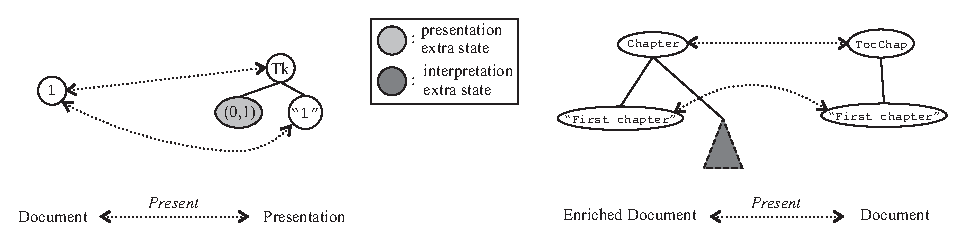
\epsfig{file=pics/eps/presIntrESExamples.eps, width=125mm}
\end{center}
\caption{Two examples of extra state.} \label{layerExtraState} 
\end{center}
\end{figure}

% example intr extra

The right-hand side of Figure~\ref{layerExtraState}\note{don't use Extra and \Core already in this figure} shows an example of {\em interpretation extra state}: a word processor with an editable table of contents view. A document level chapter is presented only partially on the enriched document level, since the content of the chapter is left out. For sake of simplicity, we assume that the enriched document only contains the table of contents and not the chapters themselves. This way, we only have to consider the extra state here and not the duplication (titles appearing in the table of contents as well as in the chapters). Section~\ref{mappingsInLayer} discussed how to handle duplications in general, and the same method can be used for the table of contents.

On reduction, the table of contents is mapped back onto a complete document, including the shaded content parts that are not in the enriched document. The title of a chapter comes from the entry in the enriched document, whereas the content is reused from the chapter of which the entry is the presentation. 

\note{mention that intr ES is more important then pres ES here?}


% even with pres, there can still be extra state
Even if an element $E_H$ is mapped onto one or more elements $E_{L,0\dots n-1}$  in the other level, it can still be part of the extra state if the elements $E_{L,0\dots n-1}$ do not constitute enough information to compute $E_H$. Consider for example a presentation of a Haskell source, in which al integers are presented with the string \verb|{Int}|. The integer nodes do have a presentation, but since it does not contain enough information for the backward mapping, the integer nodes are in interpretation extra state. \note {Is this also the case for focus?} \note{Don't know much about this kind of ES yet}
%%%

An important point to note is that extra state with regard to a certain mapping, is extra state for the {\em result} type of the mapping. Hence, presentation extra state for a presentation mapping between $\Level_{H}$ and $\Level_{L}$ is in $\Level_{L}$. Vice versa, interpretation extra state is in $\Level_{H}$.

\bc Although the term presentation extra state of $\Level_i$ may suggest that this concerns state that is used during the presentation of $\Level_i$, this is not the case. The extra state of $\Level_i$ refers to the extra state with regard to the presentation of the level above ($\Level_{i-1}$) on level $\Level_i$. The only extra state that is involved in the presentation of $\Level_i$ is that of its lower neighbor: $\Level_{i+1}$
\ec


%																
\subsection{One level has two kinds of extra state} \label{sect:oneLevelDoubleES}

% One level: two kinds of extra
Figure~\ref{layerExtraState} only shows one layer, but since each data level except the document and the rendering is in between two layers, each level between the document and the rendering has two kinds of extra state. Figure~\ref{levelExtraState} shows a data level between two layers. In the medium level, a shaded left or right half denotes that an element is extra state. Elements with a shaded left half are presentation extra state for the higher layer, and elements with a shaded right half are interpretation extra state for the lower layer. Extra state in one direction is independent of extra state in the other direction, hence an element in the figure can have zero, one, or two shaded halves.

\begin{figure}
\begin{center}
\begin{center}
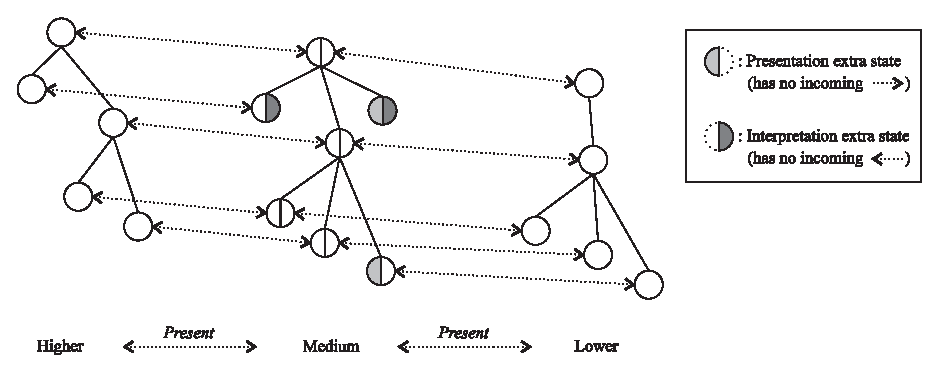
\epsfig{file=pics/eps/3levelES.eps, width=125mm}
\end{center}
\caption{Presentation and interpretation extra state in one level.}\label{levelExtraState} 
\end{center}
\end{figure}

% example one level independence of es
The whitespace extra state in tokens provides an example of the fact that extra state in one direction is independent of extra state in the other direction. As explained, whitespace is presentation extra state of the presentation level, since it cannot be computed when presenting the enriched document. On the other hand, when scanning, whitespace in tokens is computed from strings and line breaks in the layout level. Hence, whitespace is not interpretation extra state of the presentation level.

\bc
When the scanner layer interprets the layout level, spaces and row transitions between a token's string and the preceding token's string are encoded as whitespace information in the token. Since it can be computed during interpretation, the whitespace is not part of the interpretation extra state. On the other hand, when the enriched document is presented on tokens in the presentation level, the whitespace information cannot be computed, and hence it is part of the presentation extra state of the presentation level.
\ec

\note{also example of one level with both kinds of extra state? Will be somewhat contrived}
%Example Decl, Decl Type Exp., Tree view
%So always Info Pres and Intr. bla core extra:

% equations:
More specifically a data level ($\Level_{i}$) can be viewed in two ways, depending on the direction of the mapping function of which it is the result. When coming from the higher layer, the level can be considered as the product of a core part ($\Core_{\Pres,i}$) and the presentation extra state ($\Extra_{\Pres,i}$), whereas when coming from the lower layer, it is the product of a core part together with interpretation extra state (ie. $\Core_{\Intr,i} \times \Extra_{\Intr,i}$). The document and rendering level form special cases. The document ($\Level_0$) is never the result of a presentation, and therefore has no presentation extra state, whereas the rendering ($\Level_n$), which is never the result of an interpretation, has no interpretation extra state.

The specification of the data level types reads:

% Note that pres es for level i is important for pres of level i-1
% and intr es for level i is important for intr of levl i+1
\begin{small}
\refstepcounter{specification} \label{spec:levelMultiFirst}
\(\begin{array}{lcll}
\Level_{0} & = & \Core_{\Intr,0} \times \Extra_{\Intr,0}      & \text{\{Document\}}\\
\Level_{n} & = & \Core_{\Pres,n} \times \Extra_{\Pres,n}      & \text{\{Rendering\}}\\
\lefteqn{\forall i:1 \le i \le n-1:}  \\
\Level_{i}  & = & \Core_{\Pres,i} \times \Extra_{\Pres,i}     & \text{\{Viewed from higher layer\}}\\
                & = & \Core_{\Intr,i} \times \Extra_{\Intr,i} &  \text{\{Viewed from lower layer\}}\\
\end{array}\)\end{small}
\begin{center}(Specification \thespecification: Level types with extra state (Multiple layers, First attempt))\end{center}\vspace{1em}

Note that the representation of a level type as a product is only used to show that the type consists of two kinds of information. In an implementation, a level type does not need to be a product of the core and the extra state. It is likely that a level type is a tree that contains the core elements as well as the extra state elements.

We can use a simplified version of this specification in this chapter, because here we focus on a single layer only. Thus, we can drop several subscripts and for each adjacent level ($\Level_{H}$ and $\Level_{L}$) only consider one of the views from Specification~\ref{spec:levelMultiFirst}, thereby improving readability of the layer specification that will be presented further on. 

From the perspective of a single layer with its adjacent data levels, we only need to consider the upper level interpretation extra state, and lower level presentation extra state. The upper level presentation extra state as well as the lower level interpretation extra state level are handled by adjacent layers. Hence, $\Level_{H}$ and $\Level_{L}$ no longer need two views. Furthermore, the document and rendering levels are no longer special cases, since by definition the document cannot be a lower level and the rendering cannot be a higher level. The simplified equations are:

\begin{small}\( \begin{array}{lcll}
\Level_{H} & = & \Core_{\Intr, H} \times \Extra_{\Intr, H}\\
\Level_{L} & = & \Core_{\Pres, L} \times \Extra_{\Pres, L}\\
\end{array}\)\end{small}

Finally, because each level now only has one kind of extra state, we can drop the $\Pres$ and $\Intr$ subscripts, yielding:

\begin{small}
\refstepcounter{specification} \label{spec:levelSingleFirst}
\( \begin{array}{lcll}
\Level_{H} & = & \Core_{H} \times \Extra_{H}\\
\Level_{L} & = & \Core_{L} \times \Extra_{L}\\
\end{array}\)\end{small}
\begin{center}(Specification \thespecification: Level types with extra state (Single layer, First attempt))\end{center}


%																
\subsection{Mapping information} \label{sect:mappingInformation}

When a level is updated and subsequently presented or interpreted, yielding a target level that contains extra state, the extra state from the previous value for the target level must be reused. However, the new value of the target level together with its previous value do not provide sufficient information for reusing the extra state. For example, when a list of integers that is presented as a list of tokens with whitespace, has been reordered, the tokens in the whitespace must be reordered correspondingly.  In order to do so, the layer needs to keep track of additional information about the mapping.

For each target level node that is not extra state, we keep track of its origin in the source level. Thus, when presenting a higher level ($\Level_{H}$), each node in the presentation ($\Level_{L}$) contains a reference to the higher level node from which presentation it is a part. Similarly, when interpreting a lower level, each resulting $\Level_{H}$ node has references to the lower level nodes of which it is the interpretation. 

We introduce two types for this mapping information: $\Info\idwn_{H}$ denotes the {\em interpretation mapping information} in the higher level (pointing to the lower level), and $\Info\iup_{L}$ denotes the {\em presentation mapping information} in the lower level (pointing to the higher level). Similar to the $\Core$ and $\Extra$ types, the $\Info$ types are only conceptual and do not necessarily correspond to types in an implementation. Figure~\ref{coreExtraInfoExamples} shows the two examples from Figure~\ref{layerExtraState} with explicit mapping information arrows. \note{Figure is not entirely right yet, non shaded can be high or low.}

\begin{figure}
\begin{center}
\begin{center}
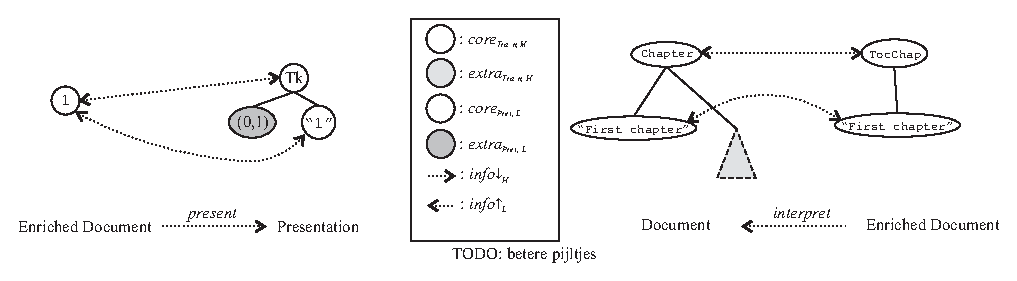
\epsfig{file=pics/eps/coreExtraInfoExamples.eps, width=125mm}
\end{center}
\caption{Two extra state examples with explicit mapping information.}\label{coreExtraInfoExamples} 
\end{center}
\end{figure}

Because the mapping information is part of a level, we define the level type to be a product of $\Info$ and 
$\Extra \times \Core$. Except for the top and bottom levels, all levels contain presentation and interpretation information. The top level is never the result of a presentation mapping, and hence has no presentation information ($\Info\iup$), whereas the bottom level has no interpretation information ($\Info\idwn$). The new definition of $\Level_i$ is:

\begin{small}
\refstepcounter{specification} \label{spec:levelMultiFinal}
\begin{align*}% \label{sse}
\end{align*} 
\(\begin{array}{lcll}
\Level_{0} & = & \Core_{\Intr,0} \times \Extra_{\Intr,0} \times \Info\idwn_{0} \\
\Level_{n} & = & \Core_{\Pres,n} \times \Extra_{\Pres,n} \times  \Info\iup_{n}\\
\lefteqn{\forall i:1 \le i \le n-1:}  \\
\Level_{i} & = & \Core_{\Pres,i} \times \Extra_{\Pres,i}  \times \Info\iup_{i} & \text{\{Viewed from upper layer\}}\\  
               & = & \Core_{\Intr,i} \times \Extra_{\Intr,i} \times \Info\idwn_{i} & \text{\{Viewed from lower layer\}}
\end{array}\)\end{small}
\begin{center}(Specification \thespecification: Level types (Multiple layers, Final))\end{center}\vspace{1em}

Note that for the middle levels, for which two kinds of mapping information exist, each alternative of the definition only contains one kind. This is because the downward mapping information $\Info\idwn_{i}$ cannot be computed by the higher layers presentation mapping, and hence is part of its extra state: $\Extra_{\Pres,i}$. Analogously, viewed from the lower layer, $\Info\iup_{i}$ is part of $\Extra_{\Intr,i}$. Rather than further complicating the definition by splitting the extra state type in a mapping information part and a regular extra state part (eg. $\Extra_{\Pres,i} = \Extra_{\mathit{Regular},\Pres,i} \times \Info\idwn_{i}$), we choose to make explicit only the mapping information relevant for the direction from which the level is viewed.

Again, the definition can be simplified by taking a single layer perspective. Note that we leave the arrows in the  mapping information types, even though they are redundant now.

\begin{small}
\refstepcounter{specification} \label{spec:levelSingleFinal}
\(\begin{array}{lcll} \label{spec:extraStateSL}
\Level_{H} & = & \Core_{H} \times \Extra_{H} \times \Info\idwn_{H}\\
\Level_{L} & = & \Core_{L} \times \Extra_{L} \times \Info\iup_{L}\\
\end{array}\)\end{small}
\begin{center}(Specification \thespecification: Level types (Single layer, Final))\end{center}\vspace{1em}

\bc
% example in picture 
Figure~\ref{mappingInfo} shows two examples of the $\Info$ argument. The left-hand side shows the situation at the presentation layer of a Haskell source editor during presentation.  The enriched document element \verb|If|  was presented on the three tokens in the presentation level. The downward arrows represent $\Info_{\Pres,H}$, whereas the upward arrows are the interpretation information $\Info_{\Intr, L}$. The dotted arrows represent $\Info_{\Intr,H}$ (upward) and $\Info_{\Pres,L}$ (downward), which are not used in this layer. The whitespace nodes in the presentation level are presentation extra state, that has to be reused on presentation. \note{more detail on reuse?}

The right-hand side of the figure shows the evaluation layer of a word processor during interpretation. The document is a \verb|Chapter| element containing two \verb|Section| children, which is mapped onto a table of contents structure in the evaluation level. Again, downward arrows are $\Info_{\Pres,H}$ and upward arrows are $\Info_{\Intr,L}$. \note{mention there is no $\Info_{\Intr,H}$?} In this case, the document contains interpretation extra state, since the contents of the chapter and sections cannot be computed from the enriched document.  \note{more detail on reuse?}

\begin{figure}
\begin{center}
\begin{center}
\begin{footnotesize}
\begin{verbatim}
Enriched Document:                       Document:                                                                                            
                                                                                            
                  If                         Chapter "chapter 1" {"this is bla bla bla..."} 
            / /   | |   \\                      v       v                                     
           v v    v v    vv              Sect "1" {"..."}     Sect "2" {"..."}                
       ^           ^           ^           |   /                    \   |                            
      /    ^       |   ^        \  ^       v  v          ^  ^        v  v                          
    Token /      Token |      Token \                    |  |                             
 {WS} "if"    {WS} "then"  {WS} "else"      ChapterTocEntry "chapter 1"                     
                                          ^              ^                 ^   ^              
Presentation:                            SectionTocEntry "1"  SectionTocEntry "2"           
                                                                                            
                                         Enriched Document:                                 

----------                                                                        
legend   ^ is pres info       v is intr info     {node} is extra state            
                                                                                  
\end{verbatim}  
\end{footnotesize}                                                                  
\end{center}                                                                      
\caption{Mapping information.}\label{info}                          
\end{center}                                                                      
\end{figure}

%??? 
%Mapping is to the node for reusing. Mapping to path is for associating doc edits with presentation parts.
%If things are moved, the paths are no longer meaningful (nodes are). Before doc op, always fix paths by parsing.


%What about keeping list [ID->Info?] that switches and is not part of level.
We choose to make the mapping information part of the $\Level$ type. The reason for this is that both adjacent layers may update a level, and therefore also affect the mapping information on the level. \note{need an example? ** Johan: ja **} With the mapping information in the level types, $\present$ and $\interpret$ do not need additional arguments anymore.
\ec



%																
%																
%																
\section{Maintaining the presentation invariant during editing} \note{are we really maintaining an invariant?}  \label{sect:maintainingInv}

The abstract functions $\Present$ and $\Interpret$ from the previous section specify what values need to be computed when a level is updated, but do not specify how the values are computed, since the functions are abstract and cannot be evaluated. In this section, we develop a number of concrete  functions that implement the behavior of the abstract functions.

\begin{figure}
\begin{center}
\begin{center}
\epsfig{file=pics/eps/maintain.eps, height=45mm} \epsfig{file=pics/eps/maintainSheet.eps, height=45mm}
\end{center}
\caption{Maintaining the invariants: without sheets (left) and with sheets (right)}\label{maintainingInvs} 
\end{center}
\end{figure}\note{Split the figure because rhs is used in different subsection?}

First, we start with two functions $\present$ and $\interpret$ that directly implement $\Present$ and $\Interpret$. The left-hand side of Figure~\ref{maintainingInvs} shows how the abstract and concrete functions are related. The precondition is that the lower level is a correct presentation of the higher level. When the lower level is updated as a consequence of a user edit, a new higher level is computed by $\interpret$, establishing the interpretation invariant. Subsequently, when the higher layers have computed a final value for the higher level, $\present$ computes a final lower level value, establishing the presentation invariant. The functions $\Edit$ and $\Transform$ are left abstract until the layers are connected in Chapter~\ref{chap:layeredArchs}.

In the figure, values that are input or output values to the layer have a special notation. The other values are either constants or intermediate values in the computation. The input and output values are used as the basis for connecting the layers in Chapter~\ref{chap:layeredArchs}. Two kinds of data flow can be distinguished: horizontal data flow between edit steps, and vertical data flow between layers.

In this first approach, the results of the previous edit step 
($\level_{H}$ and $\level_{L}$), are not used by any concrete function yet, and therefore are not really input to the layer. However, as we extend the specification to handle extra state $\level_{H}$ is used, and for the incremental model in Section~\ref{sect:maintainingInc} both levels are necessary.

We can specify the computation with equations, yielding a still rather uninformative specification, since the mapping functions $\present$ and $\interpret$ are assumed to directly implement their abstract counterparts. This direct specification will serve a starting point for further refinements.

\begin{small}
\refstepcounter{specification} \label{spec:immediate}
\begin{math} 
\interpret	::  \Level_{L} \rightarrow \Level_{H} \hfill ~\\
\present	:: \Level_{H} \rightarrow \Level_{L}  \hfill ~\\
\level_{L} = \Present~\level_{H}		\hfill \text{\{Precondition\}}\\
\level'_{L} = \Edit~\level_{L}			\hfill\text{\{User edit\}}\\
\level'_{H} = \interpret~\level'_{L} \hfill \text{\{Compute new higher level\}}\\
\level'_{H} = \Interpret~\level'_{L}		\hfill \text{\{Intermediate condition\}}\\
\level''_{H} = \Transform~\level'_{H}	\hfill \text{\{Higher layer update\}}\\
\level''_{L} = \present~\level''_{H} 	\hfill \text{\{Compute new lower level\}}\\
\level''_{L} = \Present~\level''_{H}		\hfill \text{\{Postcondition\}}\\
\end{math}\end{small}\\
\begin{center}(Specification \thespecification: Direct implementation of $\Interpret$ and $\Present$)\end{center}\vspace{1em}

In order to give a more detailed specification, and also because the presence of extra state makes it difficult to directly implement the abstract functions, we refine the specification in the next sections. Section~\ref{sect:maintainingSheet} adds style sheets to $\present$ and $\present$, Section~\ref{sect:maintainingExtraState} adds support for extra state handling, and finally Section~\ref{sect:maintainingInc} specifies an incremental version of the mapping functions.


%																
%																
%																
\subsection{Presentation and interpretation sheets} \label{sect:maintainingSheet}

The first refinement we make is the addition of $\sheet$ parameters to $\present$ and $\interpret$. In specification~1, the presentation of the higher data level depends only on the higher level itself and the presentation mapping. The same holds for the interpretation. However, we may wish to specify separately how a level is presented without altering the data level or using a different presentation mapping. Therefore, we parameterize the presentation and interpretation functions with style sheets that specify how data levels are to be represented and interpreted (also see Section~\ref{sect:archProximaLayers}). The right-hand side of Figure~\ref{maintainingInvs} shows a graphical representation of the computation after style sheets have been added. \note{more info on what style sheets are?}

The presentation sheet has the abstract type $\Sheet_{\Pres}$, and the interpretation sheet is of type $\Sheet_{\Intr}$. The equations thus become:

\begin{small}
\refstepcounter{specification} \label{spec:sheets}
\( \begin{array}{lcll}
\interpret &::& \Sheet_{\Intr} \rightarrow  \Level_{L} \rightarrow \Level_{H} \\
\present &::& \Sheet_{\Pres} \rightarrow  \Level_{H} \rightarrow \Level_{L} \\
\level_{L} & = & \Present~\level_{H}					& \text{\{Precondition\}}\\
\level'_{L} & = & \Edit~\level_{L}						& \text{\{User edit\}}\\
\level'_{H} & = & \interpret~\sheet_{\Intr}~\level'_{L}	& \text{\{Compute new higher level\}}\\
\level'_{H} & = & \Interpret~\level'_{L}					& \text{\{Intermediate condition\}}\\
\level''_{H}& = & \Transform~\level'_{H} 					& \text{\{Higher layer update\}}\\
\level''_{L} & = & \present~\sheet_{\Pres}~\level''_{H}    & \text{\{Compute new lower level\}}\\
\level''_{L} & = & \Present~\level''_{H}					& \text{\{Postcondition\}}\\
\lefteqn{\interpret~\sheet_{\Intr} \oo \present~\sheet_{\Pres} = id_{H}} & & & \text{\{***add this one?***\}}\\
\end{array}\)\end{small}\\
\begin{center}(Specification \thespecification: Support for presentation and interpretation sheets)\end{center}\vspace{1em}
\note{also put id condition in previous invariant? And add the PRES INTR one too?}

The presentation sheet for the presentation layer specifies the presentation of the enriched document. At the evaluation layer, the presentation sheet is called the evaluation sheet, which specifies the computation of the derived values. The interpretation sheet at the presentation level specifies the parser, and at the evaluation layer it specifies the reducer, which maps updates on derived structures back onto updates on the document. Note that the sheets do not appear in the abstract $\Present$ and $\Interpret$ functions, as these functions represent the intended presentation and interpretation mappings that we implement with the functions 
$\present$, $\interpret$ and the respecitive sheet parameters.

\note{??? mention composition = identity req.?}
Although a layer has two sheets, the two are closely related as they have to satisfy the
$\Interpret \oo \Present = id_{H}$ condition. For simple editors, the sheets at the evaluation and presentation layer may even originate from a single specification. However, we choose to represent the sheets as two separate entities because the mappings they define do not have to be the same. \note{Say this differently, of course the mappings are not the same. intr is more liberal? intr is not injective?} Furthermore, the two sheets may be specified in completely different formalisms. For example, at presentation level, the presentation of the document may be specified by an attribute grammar, whereas the parser may be specified using a combinator parser\cite{combinatorparser}.



%																
%																
%																
\subsection{Maintaining extra state} \label{sect:maintainingExtraState}

Until this section, we assumed that the mapping functions directly map one level onto another. However, in the presence of extra state (see Section~\ref{sect:extraState}), such a mapping may be difficult to implement. In this section, we give a more detailed specification of the mappings in a layer, by splitting the mapping function into two parts. The first part is a $\present$ or $\interpret$ function that maps a level onto another level without extra state, and the second part is a function that reuses the extra state from a previous value of the level. Together, the two parts form a mapping between two levels.

When taking extra state into account, we regard the type of a data level as the product of three types: 
$\Core \times \Extra \times \Info$ (see Section~\ref{sect:oneLevelDoubleES}). The $\Core$ part can be computed by the mapping function ($\present$ or $\interpret$), whereas the $\Extra$ part needs to be reused from the previous value of the level. The $\Info$ part is information on the origin of nodes in the core part. The types of $\Level_{H}$ and $\Level_{L}$ as defined in Section~\ref{sect:oneLevelDoubleES} are: 

\begin{small}\begin{math} 
\Level_{H} = \Core_{H} \times \Extra_{H} \times \Info\idwn_{H}\\
\Level_{L} = \Core_{L} \times \Extra_{L} \times \Info\iup_{L}\\
\end{math}\end{small}

We introduce new functions $\present$ or $\interpret$ that no longer map a level type onto a level type, but instead map a level type onto a core type. Besides the core, both functions also return the information on the origin of nodes in the result. The types are:

\begin{small}\begin{math}
\interpret :: \Sheet_{\Intr} \rightarrow \Level_{L} \rightarrow \Core_{H}\times \Info\idwn\\
\present :: \Sheet_{\Pres} \rightarrow  \Level_{H} \rightarrow \Core_{L}\times \Info\iup\\
\end{math}\end{small}
%***** WHAT ABOUT PRES . INTR = ID?

In order to realize a mapping between levels rather than between a level and a core, we introduce two new functions: $\reuse_{\Intr}$  and $\reuse_{\Pres}$. Both functions take the previous value of a level along with a $\Core \times \Info$ value, and return a new value for the level, containing the $\Core \times \Info$ from the argument, together with the $\Extra$ from the previous value of the level. In case $\Extra$  cannot be reused, a default value is used. The types of the $\reuse$ functions are:

\begin{small}\begin{math}
\reuse_{\Intr} ::  \Level_{H} \rightarrow \Core_{H} \times \Info\idwn_{H} \rightarrow \Level_{H}\\
\reuse_{\Pres} ::  \Level_{L}  \rightarrow \Core_{L} \times \Info\iup_{L}    \rightarrow \Level_{L}\\
\end{math}\end{small} \note{does reuse need the other level as well?}

The composition of a mapping function and a reuse function yields a mapping between levels. For example, for the interpretation, we get:

\begin{small}\begin{math}
\reuse_{\Intr}~\level_{H} \oo \interpret~\sheet_{\Intr} :: \Level_{L} \rightarrow \Level_{H}
\end{math}\end{small} \note{does reuse need the other level as well?}

Note that the strict separation between a mapping function and its corresponding reuse function is for specification purposes only. In general, it is not possible to reuse extra state from only the core value and the previous value of the level. For example, for the interpretation direction, the mapping information in the lower level ($\Info\iup_{L}$) is required in order to reuse higher level extra state. However, the result of 
$\interpret$ has type $\Core_{H}\times \Info\idwn$ and does not contain the required information. Simply passing $\Info\iup_{L}$ to $\reuse_{\Intr}$ is not an option, because the information is about the mapping between $\Level_{L}$ and $\Level_{H}$ and not about the mapping between $\Core_{H}$ and $\Level_{H}$.\note{give an example here?} An implementation will combine $\interpret$ with ${\tt reuse_{\Intr}}$ and use the $\Info\iup_{L}$ information to reuse the higher level extra state while computing the interpretation. The same thing holds for the presentation.


\bc
 An example shows why It is in general not possible to reuse the extra state from only the core value. Passing $info$
For example, consider a list of declarations {\tt [ Decl "f" $exp_f$, Decl "g" $exp_g$]} that is presented as a list of string tokens: {\tt ["f", "g"]}. The presentation does not contain the right-hand sides of the declarations, which are therefore interpretation extra state of the enriched document. This means that when parsing the identifier list, the right-hand sides $exp_f$ and $exp_g$ cannot be computed, and have to be reused. 
The right-hand sides of the declarations are not presented, and therefore cannot be computed during parsing. in the presentation, and therefore the table of contents T
An example to clear it up:
 make the specification clear. 
 reuse present and interpret already need to be special. Otherwise not possible to reuse. For example, consider a list of declarations that is presented as a li when list [Decl "f" <Exp>, Decl "g"] is mapped onto list of tokens ["f", "g"]. When parsing this list, exps are ES. Now, if f and g are swapped, parsing gives [Decl' "g", Decl' "f"],  reuse must now fix the exps. Not possible if parse does not keep extra information.
\ec

Figure~\ref{maintainExtraState} shows how the invariants are maintained when taking extra state into account. The figure is similar to the right-hand side of Figure~\ref{maintainingInvs}, but both $\present$ and
 $\interpret$ are composed with an appropriate $\reuse$ function. The ovals around the compositions reflect the conceptual nature of the separation between the mapping and reuse functions. \note{say that $\Level_H$ is now an input?}
\note{what about level''H, it is both input (vertical) and output (horizontal)}

\begin{figure}
\begin{center}
\begin{center}
\epsfig{file=pics/eps/maintainES.eps, width=125mm}
\end{center}
\caption{Maintaining the invariants in the presence of extra state.}\label{maintainExtraState} 
\end{center}
\end{figure}

%Because the higher level is a parameter to $\reuse_{\Intr}$, it . The level at the top right of the figure %($\core''_{H} \times extra''_{H} \times info''\idwn_{H}$) is somewhat special, since it is both an input as well as an %output value of the layer. It is an input value, because it is computed by the upper layer, but 


The specification of the computation now reads: \note{explain more?}

\begin{small}
\refstepcounter{specification} \label{spec:extraState}
\begin{math} 
\text{\bf type}~\Level_{H} = \Core_{H} \times \Extra_{H} \times \Info\idwn_{H}\\
\text{\bf type}~\Level_{L} = \Core_{L} \times \Extra_{L} \times \Info\iup_{L}\\
\interpret :: \Sheet_{\Intr} \rightarrow \Level_{L} \rightarrow \Core_{H} \times \Info\idwn_{H}\\
\present :: \Sheet_{\Pres} \rightarrow  \Level_{H} \rightarrow \Core_{L} \times \Info\iup_{L}
\end{math}\\
\( \begin{array}{rcll} 
\level_{L} & = & \Present~\level_{H}						& \text{\{Precondition\}}\\
\level'_{L} & = & \Edit~\level_{L}							& \text{\{User edit\}}\\
\core'_{H} \times info'\idwn_{H} & = &\interpret~\sheet_{\Intr}~\level'_{L}	& \text{\{Compute new higher core\}}\\
\level'_{H} & = & \reuse_{\Intr}~\level_{H}~\core'_{H}\times info'\idwn_{H} & \text{\{Reuse extra state\}}\\
\level'_{H} & = &\Interpret~\level'_{L}						& \text{\{Intermediate condition\}}\\
\level''_{H} & = & \Transform~\level'_{H} 					& \text{\{Higher layer update\}}\\
\core''_{L} \times info''\iup_{L} & = & \present~\sheet_{\Pres}~\level''_{H}		& \text{\{Compute new lower core\}}\\
\level''_{L} & = & \reuse_{\Pres}~\level_{L}~\core''_{L} \times info''\iup_{L} & \text{\{Reuse extra state\}}\\
\level''_{L} & = & \Present~\level''_{H}						& \text{\{Postcondition\}}\\
\end{array}\)\end{small}
\begin{center}(Specification \thespecification: Support for extra state)\end{center} 
\vspace{1em}

% computation order
The $\Info\idwn_{H}$ mapping information used by $\present$ is computed by $\interpret$ and vice versa. As a consequence, at a single level only one kind of mapping information is guaranteed to be valid; after presentation, the interpretation mapping is correct, but the presentation mapping may be incorrect, whereas after interpretation, the presentation information is correct, but the interpretation information may be incorrect. However, this is not a problem since a level is presented before its lower neighbor is interpreted, and vice versa. 
%\note{when we have higher level edit ops, this will become a problem}

% maak para duidelijker
It may seem more appropriate that presentation mapping information ($\Info\idwn_{H}$) is a result of the presentation, rather than the interpretation, since it concerns information about the presentation of the level and not about its interpretation, but this is not the case. Firstly, the presentation mapping information is part of the higher level, whereas $\present$ returns the lower level. Hence in order to return $\Info\idwn_{H}$, $\present$ would have to return both higher and lower level data.  Furthermore, after a level is presented, the lower level may be updated by the layer below. If $\present$ computes $\Info\idwn_{H}$, which refers to the lower level, then this information may not be correct anymore after a lower level update. By computing the mapping information on interpretation, the problem is avoided, since after it is interpreted, the lower level is not edited before the higher level is presented again. For a similar reason, $\Info\iup_{L}$ is computed by $\present$.

\note{does give a problem when mappings are not inverse}
\note{eg. "chess:" "board" -> ChessBoard. Now ChessBoard has wrong pres info when presented on an image instead of tokens}
% if pres.interpret not is id, then interpret map is different from pres map. 
% ES is not valid. interpret.pres is always id


\bc CRAP:
% mapping we have is not good enough
The available mapping functions $\present$ and $\interpret$ both implement from $\Level$ to $\Core$, whereas the layer needs to realize mappings from level to level. Hence, we introduce a function reuse, that restores However, the editor layer has to realize mappings between levels, and hence we need functions $\present$ and $\interpret$ that have a result type of $\Core \times \Extra$:
% not for top and bottom

% what extra  vv wrong: not an argument
The $\Extra$ information in the result types cannot be computed from the arguments. Instead, we try to reuse its previous value. In order to do so, $\interpret$ and $\present$ get an extra argument which, for each node, contains the nodes it was previously mapped onto. For $\interpret$, the extra argument is of type $\Info_{\Intr}$, and it is computed by $\present$. Analogously, $\present$ gets an extra argument of type $\Info_{\Pres}$, which is computed by $\interpret$. \note{already mention computation order here?}
\ec

%																
\subsection{Safety of extra state}

Because the reuse of extra state depends on the mapping information, extra state may be lost if the mapping information is not valid. There are two ways in which the mapping information can become invalid.  

The first situation occurs when a level is updated in such a way that the mapping information computed at the previous presentation or interpretation, is no longer correct. An example is when a document edit operation in a Haskell source editor changes a sum to a product. The old presentation mapping in invalid, since it points to the presentation of the sum. In this case, because of the similarity between the presentations of a sum and a product, the tokens can be reused, but if the updated node has a completely different presentation, then the layout information of the tokens is lost. \note{this is the higher level edit op problem}

The second situation in which the mapping information may be invalid, is if 
$\present \oo \interpret$ is not the identity function for a node. \note{say this some other way?} An example is found in a source editor that provides graphical presentations for some of its tokens (eg. $\rightarrow$ for the token \verb|"->"|). If a \verb|"->"| token is parsed, the mapping information in the resulting enriched document node points toward the textual arrow. However, if the enriched document is presented, the presentation contains a graphical arrow, and hence the mapping information with respect to the arrow token is incorrect. In such a case, the editor designer must take care of reusing extra state from the textual arrow token for the graphical arrow token. The reverse situation does not occur, since we require that $\interpret \oo \present$ is identity for a node. \note{do we?}

In case the extra state cannot be restored, it is set to a default value. Thus, if an entry is added to a table of contents in the enriched document of a word processor, an empty chapter (or section) added to the document. Similarly, if a document edit operation in a source editor adds a new structure to the document, its presentation gets a default layout.

The responsibility for restoring extra state and handling problematic situations lies within each layer itself. Restrictions on the presentation and interpretation mappings may guarantee the safety of extra state, but currently, no such restrictions have been established. However, the fact that safety of extra state cannot be guaranteed in general, does not necessarily pose a problem. Since presentation extra state generally consists of non-essential information, it is not a big problem that in some rare cases, it is reset to a default value. \note{mention this difference somewhere before?} Interpretation extra state, on the other hand, does represent essential information, but by restricting the edit behavior on presentations that have interpretation extra state, it can be protected. For example, the edit behavior on a table of contents can be restricted to updates on titles, and insertion and deletion of entire entries. For these edit operations, the desired effect on the document is clear, and the situation that extra state cannot be reused is avoided. If the editor supports the behavior that deleting entries from the table of contents causes deletion of the corresponding sections, then a warning can be issued that the deletion affects more than the focused part of the enriched document. 

\note{can we always tell that extra state was lost?}

%Now left to editor. During pres, do we have old node? And what about intr? Do we have old pres?
%Would be nice if we could guarantee safety. When? context free presentation?
%list delete is in general no problem  Or parent if context sensitive presentation.

%higher level update without lower level interpretation gives problem. but not mentioned here, only in layered archs
%lower level update without higher level pres?   is this not just editing and skipping higher layers?


%																
\subsection{Conclusions}

\bc seems a bit overdone to repeat the spec here.
% the final spec

specification, not equations
The equations that describe the behavior of $\present$ and $\interpret$ in the presence of extra state are:

\begin{small}\begin{align*}% \label{sse}
\interpret_{i} :: \sheet_{\Intr,i} \rightarrow \Level_{i+1} \rightarrow \Level_{i}\\
\present_{i} :: \sheet_{\Pres,i}  \rightarrow  \Level_{i} \rightarrow \Level_{i+1}\\
\\
%\level_{L} = \Present~\level_{H}\hfill \text{\{Precondition\}}\\
\level'_{H} = \interpret~\sheet_{\Intr}~\level'_{L}\\
%\level'_{H} = \Interpret~\level'_{L}\hfill \text{\{Intermediate condition\}}\\
\level''_{L} = \present~\sheet_{\Pres}~\level''_{H}\\
%\level''_{L} = \Present~\level''_{H}\hfill \text{\{Postcondition\}}\\
\interpret~\sheet_{\Intr}  \oo \present~\sheet_{\Pres} = id_{H}\\
\\
\Present_{i} :: \Level_{i} \rightarrow \Core_{\Pres,i+1}\\
\Interpret_{i} :: \Level_{i+1} \rightarrow \Core_{\Intr,i}\\
\end{align*} 
\end{small}
\center{()}
\ec


The model for extra state presented in this section only shows what information must be kept track of by a layer in order to handle extra state. It does not specify how to keep track of the extra information, nor how to reuse extra state in conflict situations. This is left as a responsibility of the individual layers. Furthermore, the proposed model of reusing extra state only handles extra state that is attached to a core parent node. \note{explain process of reusing more explicitly somewhere?} 

The model works for specifying the whitespace extra state for token presentations as well as interpretation extra state for editing partial presentations. Further research is required to established restrictions on the presentation and interpretation mappings that can guarantee safety of extra state. Furthermore, a method for handling extra state that is not attached to specific parent nodes is desirable. \note{related to n:m presentation problem} Finally, experience with building editors with Proxima, as well as using these editors will provide more instances of extra state, and information on how to resolve conflict situations.

% Not enforced by the invariants! Need more detailed stuff on element level. Future research.

%Remember ES on parsing stuff is fragile
%unless strong restrictions. important for interpretation direction
%layout is an example. things like order are harder. extra layer?
%Many possibilities not researched yet.

%Have to figure out more about Focus ES, and other non node ES.
%order changes are not yet clear!


%																
\section{Incrementality} \label{sect:maintainingInc}
% meer uitleg?: no choice on inc, even memo may be used, but do need old level for that.

In the previous section, $\present$ and $\interpret$ together with the $\reuse$ functions realize a mapping from one level to another. This means that each time a mapping is computed, the entire result level needs to be computed. However, changes in one level frequently only cause local changes in the other level. For example, if the presentation of a paragraph in a word processor is changed, the corresponding enriched document update only concerns that single paragraph. In this section, we change the mapping functions in such a way that instead of mapping one level onto another, they map an edit operation on one level onto an edit operation on the other level. \note{explain that this is at least as powerful as non-incremental? ({\tt $\backslash$(Set lvl) -$>$ Set lvl')}}

Of course, even if the presentation is a mapping between levels, it can be made incremental by using implementation techniques such as function caching. However, we choose to make the incrementality explicit. An important reason for this is that the interpretation process is more naturally understood as a process of interpreting edit operations: in a number of interpretation steps, an edit gesture provided by the user is mapped onto an edit operation on the document, or one of the intermediate levels. By modeling both directions as mappings between edit operations, the layer model becomes symmetrical. 

Because the discussion on incrementality is largely independent of extra state, we use the $\present$ and $\interpret$ mappings from Section~\ref{sect:maintainingInv} as the basis for developing the incremental mappings. Only in the final specification, we will add the explicit separation between core and extra state again.



%																
\subsection{From a mapping between levels to a mapping between edit operations}

Figure~\ref{fromLevelToOp} shows the difference between an interpretation mapping between levels and a mapping between edit operations. On the left-hand side is the mapping between levels, in which the interpretation of a new lower level yields a new higher level. On the right-hand side, a mapping between edit operations is shown. The value of an updated level is computed by applying a function
 $\update :: \Edit_\alpha \rightarrow \alpha \rightarrow \alpha$ to an edit operation and a level. A 
 $\present$ function between edit operations instead of levels can be specified similarly.  Note that we now need the previous values of both levels in order to compute the new level values.
 

\begin{figure}\begin{small}\begin{center}\begin{center}
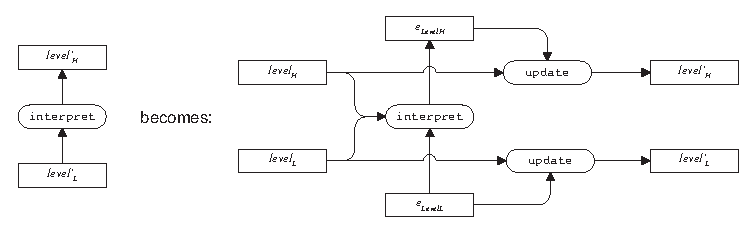
\epsfig{file=pics/eps/levelMapVsdeltaMap.eps, width=100mm}\end{center}
\caption{Level to level vs. edit operation to edit operation }\label{fromLevelToOp} 
\end{center}\end{small}\end{figure}


% there is PRES, which is a level thing, pres, which is incremental, and also presLevel
% pres will work on mappings, presLevel won't. Is this PRES? or do we keep PRES abstract
The arrows from $\Level_{H}$ and $\Level_{L}$ to $\interpret$ in the right-hand side of Figure~\ref{fromLevelToOp} are necessary because in some cases it is hard to directly map a lower level edit operation onto a higher level edit operation. \note{example?} If such a mapping is not available, but there is a non-incremental mapping between levels, then the computation sketched in Figure~\ref{computeOps} can be used to obtain a mapping between edit operations. 

The figure shows how a function $\interpret :: \Edit_{\Level_{H}} \rightarrow \Edit_{\Level_{L}}$ can be constructed when only a function with type ${\tt interpret'} :: \Level_{H} \rightarrow \Level_{L}$  is available. In the figure, an edit operation $e_{\Level_L}$ is performed on the initial lower level, using $\update$. A new higher level is then computed by applying ${\tt interpret'}$ to the updated updated lower level. Finally, the incremental higher level update is computed by taking the difference of the updated higher level and the original. In order to allow this kind of computation, $\interpret$ needs the values of the higher and lower level as arguments.

\begin{figure}
\begin{small}
\begin{center}
\begin{center}
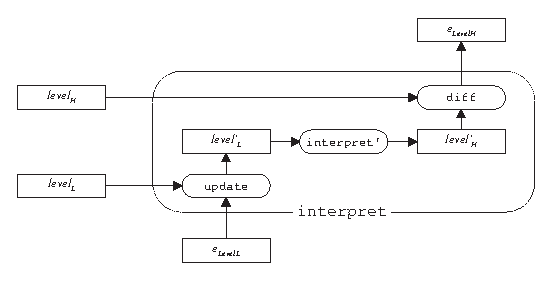
\epsfig{file=pics/eps/levelMap2deltaMap.eps, width=60mm}
\end{center}\caption{Computation of $e_{H}$ from $e_{L}$}\label{computeOps} 
\end{center}
\end{small}
\end{figure}

For the presentation mapping, a similar computation can be performed. Hence, $\present$ also needs the values of the two adjacent levels. 


%																
\subsection{Shorthand notation for level updates}

Before we give the invariants for the incremental versions of the layer functions, we introduce a shorthand notation for the $\update$ functions. Especially for larger computations, these functions clutter the diagrams, due to crossing arrows and the many rather uninformative appearances of $\update$. In the normal notation, an update $\mathit{data}' = \update~e_{\mathit{Data}}~\mathit{data}$ is represented as:\\

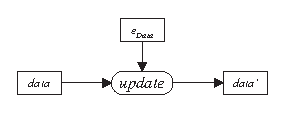
\epsfig{file=pics/eps/updateNotation.eps}

\smallskip
Because an edit operation on a value of type $\mathit{Data}$ can also be regarded as a function of type 
$\mathit{Data} \rightarrow \mathit{Data}$, we use a dashed arrow notation that leaves the function $\update$ implicit:\\

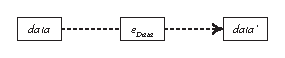
\epsfig{file=pics/eps/updateNotationShort.eps}

Figure~\ref{incrementalInterpret}, shows the right-hand side of Figure~\ref{fromLevelToOp} using the new notation.

\begin{figure}
\begin{small}
\begin{center}
\begin{center}
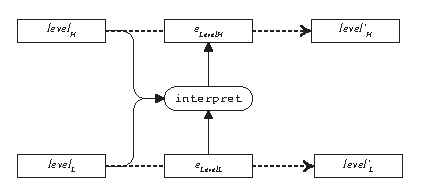
\epsfig{file=pics/eps/interpretShortNotation.eps}
\end{center}\caption{Incremental $\interpret$.}\label{incrementalInterpret} 
\end{center}
\end{small}
\end{figure}


%																
\subsection{Maintaining the presentation invariant} \label{sect:incrementalSpec}

By adding an explicit $\reuse$ function and a sheet parameter to $\interpret$ of Figure~\ref{incrementalInterpret}, and doing the same for $\present$, we obtain an incremental version of the computation specified in Section~\ref{sect:maintainingExtraState}. Figure~\ref{layerExtraStateInc} shows the incremental computation. This is the final version of the computation, which is used in the next chapter. The layer has two kinds of input and output values: the edit operations, which come from and go to upper and lower layers, and the data levels, which are the result of the previous edit step and are input to the next edit step.

\begin{figure}
\begin{center}
\begin{center}
\epsfig{file=pics/eps/maintainESinc.eps, width=125mm}
\end{center}
\caption{Maintaining the invariants incrementally.}\label{layerExtraStateInc} 
\end{center}
\end{figure}

In addition to the extra parameters, and the changes to the types of the mapping functions (now mapping edit operations instead of data levels),  the new equations for the incremental versions of $\present$ and 
$\interpret$ also contain a number of explicit  $\update$ functions: 

\begin{small}
\refstepcounter{specification} \label{spec:incrementality}
\( \begin{array}{lcl}
\text{\bf type}~\Level_{H}  =  \Core_{H} \times \Extra_{H} \times \Info\idwn_{H}\\
\text{\bf type}~\Level_{L}  =  \Core_{L} \times \Extra_{L} \times \Info\iup_{L}\\
\interpret  ::  \Sheet_{\Intr} \rightarrow \Level_{L} \rightarrow \Level_{H} \rightarrow  \Edit_{\Level_{L}} \rightarrow \Edit_{\Core_{H}\times \Info\idwn_{H}} \\
\present  ::  \Sheet_{\Pres} \rightarrow \Level_{H} \rightarrow \Level_{L}  \rightarrow \Edit_{\Level_{H}} \rightarrow \Edit_{\Core_{L}\times \Info\iup_{L}}\\
\\
\end{array}\) \\
\( \begin{array}{rcll}  
\level_{L} 	& = & \Present~\level_{H}						& \text{\{Precondition\}}\\
e_{\Level_{L}}& = & \Edit~???\level_{L}							& \text{\{User edit???\}}\\
\\
\level'_{L} 	& = & \update~e_{\Level_{L}}~\level_{L}                 & \text{\{Compute intermediate lower level\}}\\
e_{\Core_{H} \times \Info\idwn_{H}}  & = & \interpret~\sheet_{\Intr}~\level_{L}~\level_{H}~e_{\Level_{L}} & \text{\{Compute higher core update\}}\\
e_{\Level_{H}} & = & \reuse_{\Intr}~\level_{H}~e_{\Core_{H}\times \Info\idwn_{H}}     & \text{\{Reuse extra state\}}\\
\level'_{H} & = & \update~e_{\Level_{H}}~\level_{H}                 & \text{\{Compute intermediate higher level\}}\\
\\
\level'_{H} & = & \Interpret~\level'_{L}						& \text{\{Intermediate condition\}}\\
e'_{\Level_{H}} & = & \Transform~e_{\Level_{H}} 			& \text{\{Higher layer update?\}}\\
\\
\level''_{H} & = & \update~e'_{\Level_{H}}~\level'_{H}                 & \text{\{Compute final higher level\}}\\
e'_{\Core_{L}\times \Info\iup_{L}}  & = & \present~\sheet_{\Pres}~\level'_{H}~\level'_{L}~e'{\Level_{H}} & \text{\{Compute new lower core\}}\\
e'_{\Level_{L}} & = & \reuse_{\Pres}~\level_{L}~e'_{\Core_{L}\times \Info\iup_{L}} & \text{\{Reuse extra state\}}\\
\level''_{L} & = & \update~e_{\Level_{L}}~\level_{L}                 & \text{\{Compute final lower level\}}\\
\\
\level''_{L} & = & \Present~\level''_{H}						& \text{\{Postcondition\}}\\
\end{array}\)
\end{small}
\begin{center}(Specification \thespecification: Incrementality)\end{center}\vspace{1em}

Note that compared to $\interpret$, the order of the level parameters for 
$\present$ is swapped (ie. first the higher and then the lower level), since the direction of the mapping is also swapped.\note{Mention apparent mismatch with ','' on args of present and interpret now we use edit ops?} \note{user edit is weird. maybe this is not a function but some kind of constant. elow = EDIT}

Two updates take place on the higher level, and two on the lower level. However, if we look at Figure~\ref{computeOps}, we can see that a lower level update is performed in the computation of
 $\interpret$. Thus, instead of computing the updated lower level twice, an implementation of 
 $\interpret$ may perform the update itself and also return $\level'_{L}$ besides
 $e_{\Core_{H} \times \Info\idwn_{H}}$. \note{say the the remaining updates disappear because of composition?} Analogously, $\present$ may return $\level''_{H}$. \note{Mention that after composition two of the four updates can be dropped?}
 

%However, because a layer does not exist on its own, but is composed with other layers (as will be explained 
%in the next Chapter), an adjacent layer will also do an update on the level. Hence


%																
\section{Conclusions}

\toHere     % ^^^^^^^^^^^^^^^^^^^^^^^^^^^^^^^^^^^^^

In one level,  mapping info to higher and lower (except for doc \& rendering), furthermore, the tree can can be regarded bla.

-mapping for pres = Mapping pres. doc only has mapping pres, ren only mapping intr. \Core \&extra are wrt mapping of which level is destination. level is extra for pres from higher and intr from lower. Doc only has intr  and ren only pres.

A Proxima Layer:
plaatje met alle in en uitvoer van 1 level
levels from the left, updated levels to the right, and deltas up and down. In next Chapter we connect it all


Parse errors in tokens requires intr update on lower. Different model. First research necessary if this way of parsing is good



Proxima offers possibility of solving, not always solution. non tree stuff, or inserted nodes? (redundant parens, tree order) Many problems, need to be solved, but then they can be implemented.
No panacea, but at least we know where to do the difficult work. (maybe this one belongs in previous chapter?)


%																
%																
%																
%\section{Bidirectional mappings}
%
%What do we lose exactly by not keeping the mappings
%
%reuse original trees, update mappings upward and downward



%																
%																
%																
%\section{Consequences for each layer}
%Layer examples.
%In arrangement, mappings automatic, formatters etc. rest is easy
%
%In rendering, no mappings
%Doc-Pres, left to editor builder. what happens if we don't do them
%tokens contain origin in edoc. identity is reused. What if type changes?
%
%
%Using caching of parsers and presenters to preserve the mapping
%-- List support for these mappings